\section{Experimental Setup}
\label{sec:setup}
\subsection{A verification benchmark with real OCR errors}
Public OCR datasets provide images and transcriptions but no verification labels. We create them by running real OCR
engines and labelling each output against the ground truth (Figure~\ref{fig:pipeline}a), so every \textsc{Incorrect}
example is a genuine engine error, not a synthetic perturbation. Five public datasets cover four domains
(Table~\ref{tab:datasets}, Figure~\ref{fig:datasets}): \textbf{FUNSD}~\cite{jaume2019funsd}, word boxes in noisy
scanned forms (the Hugging Face release stores boxes on the LayoutLM 0--1000 grid; they must be rescaled to pixels
before cropping); \textbf{CORD}~\cite{park2019cord}, words in camera-captured receipts (official train and validation
splits form the training pool); \textbf{SROIE}~\cite{huang2019sroie}, text lines of scanned receipts, whose ground
truth is entirely upper-case, so comparison is case-insensitive; \textbf{IAM}~\cite{marti2002iam}, handwritten English
words; and \textbf{IIIT5K}~\cite{mishra2012iiit5k}, scene-text words, for which we follow the standard
case-insensitive alphanumeric protocol and give \emph{every} verifier, including \ours{} and the VLM judge, the claim in
this canonical form. Official splits are kept and pools are capped at 8{,}000 training and 4{,}000 test crops (fixed
seed). The main engine is Tesseract~5~\cite{smith2007tesseract} (LSTM, \texttt{psm 7}); on handwriting Tesseract is
degenerate (93\% word error), so IAM verifies TrOCR-small-handwritten. A second engine, TrOCR-small, is used for
engine transfer. Test error rates span 29--47\%.

\begin{table}[t]\centering
\caption{\textbf{Benchmark.} Five public datasets with real OCR errors. Error rate: share of engine outputs that differ
from the ground truth (exact match; SROIE case-insensitive; IIIT5K case-insensitive alphanumeric).}
\label{tab:datasets}
\footnotesize\setlength{\tabcolsep}{4pt}
\begin{tabular}{lllccclcc}\toprule
Dataset & domain & unit & \#train & \#test & avg.\ len. & engine & err.\ train (\%) & err.\ test (\%)\\\midrule
\tabinput{tables/datasets.tex}
\bottomrule\end{tabular}\end{table}

\begin{figure}[t]
\centering
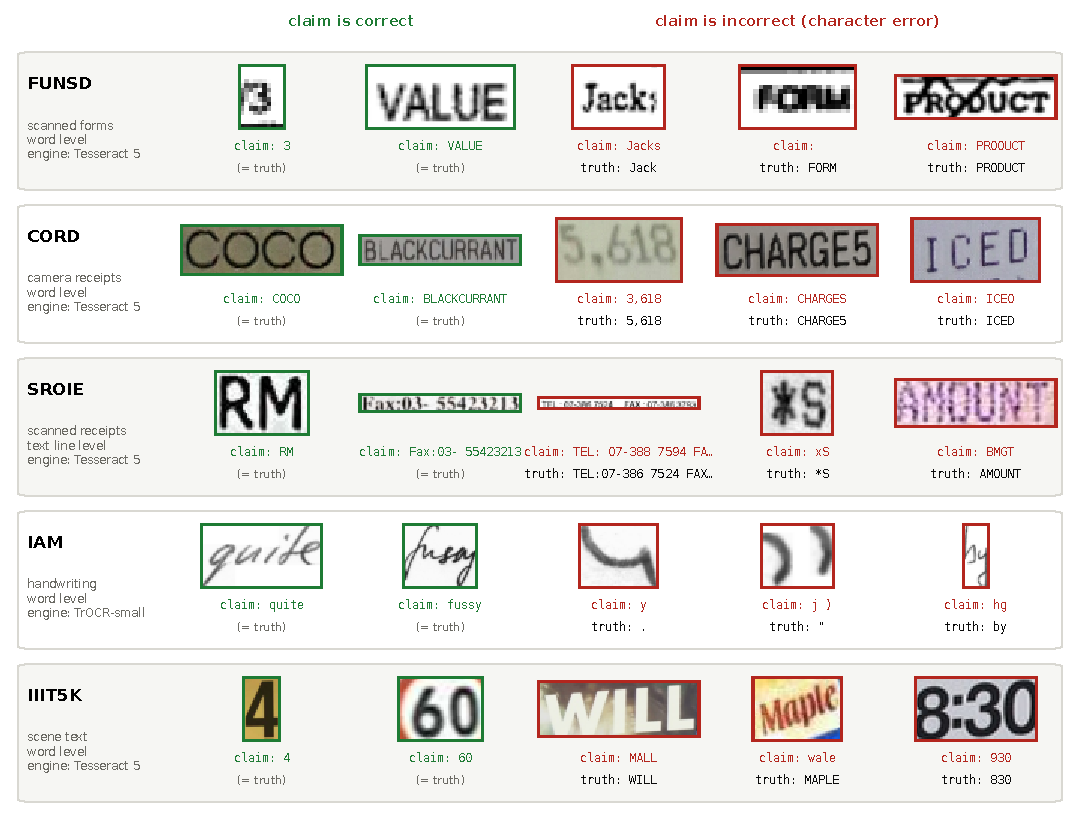
\includegraphics[width=0.9\linewidth]{figs/datasets_examples.pdf}
\caption{\textbf{The five verification benchmarks.} Real test crops with the claim of the main OCR engine, drawn by a
seeded random choice (two correct claims and three character errors per dataset; none chosen by hand). Errors range
from single confusable glyphs (\texttt{CHARGES}/\texttt{CHARGE5}, \texttt{3,618}/\texttt{5,618}) to empty or noise
outputs.}
\label{fig:datasets}
\end{figure}

\textbf{What counts as an error.} Labels inherit the datasets' conventions and noise. A share of incorrect claims
differ from the ground truth only in case or punctuation (mostly fragments of neighbouring glyphs inside the word box),
and our manual audit finds annotation errors and clipped crops among them (Section~\ref{sec:qualitative}). We keep
these claims (an engine that emits \texttt{Barbara |} for the field \texttt{Barbara} is wrong for a downstream
consumer) but also report every method on genuine character errors only (Section~\ref{sec:charerr}).
Table~\ref{tab:truth_in_graph} shows that the counterfactual graph contains the truth for 83--97\% of real errors on
printed and scene text and for 55\% on handwriting, where many errors span several characters.

\begin{table}[t]\centering
\caption{\textbf{Counterfactual graphs on the test sets}: average hypotheses per claim and share of real engine errors
whose ground truth equals TrOCR's reading, PARSeq's reading, or \emph{any} node of $G(h)$.}
\label{tab:truth_in_graph}
\footnotesize\begin{tabular}{lcccc}\toprule
Dataset & nodes & truth $=g_1$ (\%) & truth $=g_2$ (\%) & truth $\in G(h)$ (\%)\\\midrule
\tabinput{tables/truth_in_graph.tex}
\bottomrule\end{tabular}\end{table}

\subsection{Baselines, protocol and metrics}
All baselines see the same test words, and every threshold is fitted on the same $k$-shot support set as \ours{}
(maximising macro-F1). \textbf{Engine confidence}: Tesseract's mean word confidence or TrOCR-small's mean token
probability (temperature scaling is monotone and leaves ranking metrics unchanged). \textbf{ConfidNet-style learned
confidence}~\cite{corbiere2019confidnet}: an MLP trained on the support set from the engine confidence and the
verifier's likelihood statistics of the claim. \textbf{Re-recognition agreement}: accept iff an independent recogniser
reads the same string: TrOCR-base~\cite{li2023trocr}, PARSeq~\cite{bautista2022parseq} and
Florence-2~\cite{xiao2024florence}; for PARSeq we also report a \emph{graded} variant ranked by its sequence
confidence (agree $\rightarrow +c$, disagree $\rightarrow -c$), the strongest re-recognition baseline.
\textbf{Two-engine voting}: accept iff Tesseract and TrOCR-small agree. \textbf{VLM judge}:
Qwen2.5-VL-7B-Instruct~\cite{bai2025qwen25vl} asked whether the image shows exactly the claimed text, scored by
$P(\texttt{yes})/(P(\texttt{yes})+P(\texttt{no}))$ at the natural 0.5 threshold and at an \emph{oracle} threshold tuned on
the test set. \textbf{Strong learned baselines on our evidence}: logistic regression and gradient-boosted trees on
flattened LOCUS evidence and/or character evidence, DeepSets over rivals (no edges), and \ours{} from scratch.

For each $k$ we draw five class-balanced support sets (seeds 0--4); the test set keeps its natural class ratio, and we
report the ensemble of the five models. Metrics: \textbf{macro-F1} (primary), \textbf{AUROC}, \textbf{AURC} (area
under the risk--coverage curve, lower is better), \textbf{coverage@95} (share of words that can be accepted while the
accepted set stays $\geq95\%$ correct) and top-1 \textbf{repair accuracy}. In every column of a comparison table the
best entry is \colorbox{bestc}{\textbf{bold on green}} and the second best \colorbox{secondc}{\underline{underlined on
blue}}. \textbf{Implementation:} hidden size 64, 3 GATv2 layers with 4 heads, dropout 0.2; pretraining 15 epochs (AdamW,
lr $10^{-3}$, batch 64); rendering in Liberation Sans; the trainable GNN has 0.05\,M parameters and evidence extraction
runs at $\approx$18 words/s on one RTX A6000.

\begin{figure}[t]\centering
\resizebox{0.95\linewidth}{!}{% Benchmark construction (top) and deployment of LOCUS in a digitisation pipeline (bottom). No numbers.
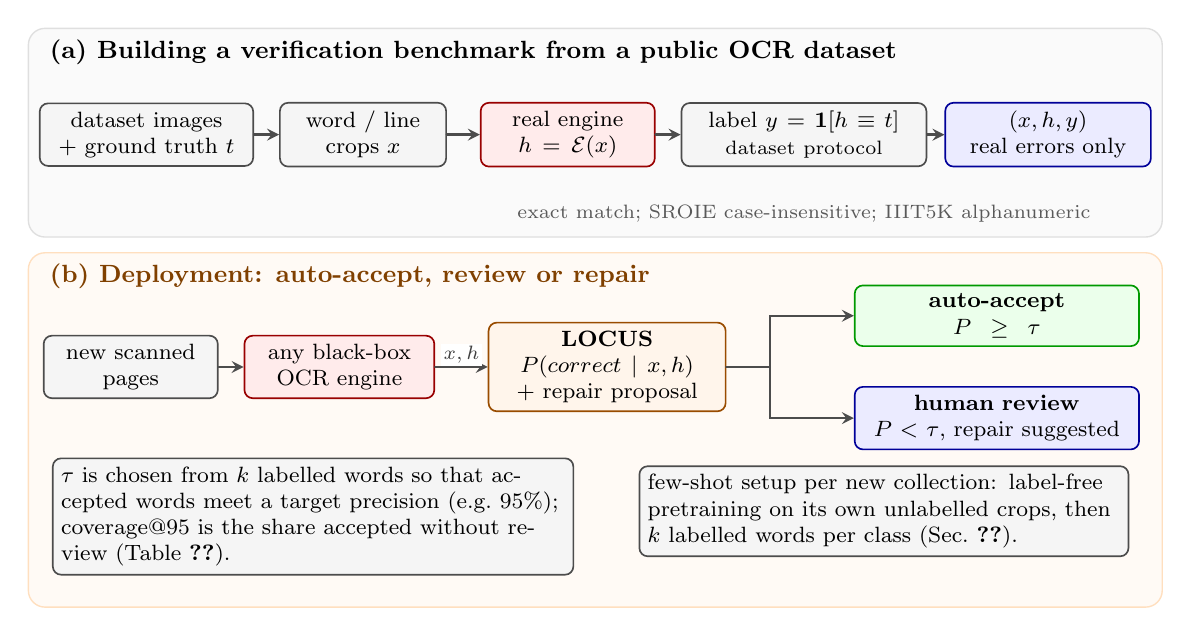
\begin{tikzpicture}[
  font=\small, >=stealth, line cap=round,
  box/.style={draw=#1!60!black, rounded corners=3pt, align=center, inner sep=3pt, fill=#1!8, line width=0.6pt, font=\footnotesize},
  box/.default=gray,
  flow/.style={->, line width=0.9pt, black!70},
  band/.style={rounded corners=6pt, fill=#1!4, draw=#1!25, line width=0.5pt},
  lbl/.style={font=\scriptsize\itshape, fill=white, inner sep=0.8pt, text=black!75},
]
\fill[band=gray]   (0,1.95) rectangle (14.4,4.6);
\fill[band=orange] (0,-2.75) rectangle (14.4,1.75);
\node[anchor=west, font=\small\bfseries] at (0.15,4.3) {(a) Building a verification benchmark from a public OCR dataset};
\node[anchor=west, font=\small\bfseries, text=orange!50!black] at (0.15,1.45) {(b) Deployment: auto-accept, review or repair};

% ---------------------------------------------------------------- (a)
\node[box, text width=2.5cm] (ds) at (1.5,3.25) {dataset images\\+ ground truth $t$};
\node[box, text width=1.9cm] (crop) at (4.25,3.25) {word / line\\crops $x$};
\node[box=red, text width=2.0cm] (eng) at (6.85,3.25) {real engine\\$h=\mathcal{E}(x)$};
\node[box, text width=2.9cm] (lab) at (9.85,3.25) {label $y=\mathbf{1}[h\equiv t]$\\{\scriptsize dataset protocol}};
\node[box=blue, text width=2.4cm] (bench) at (12.95,3.25) {$(x,h,y)$\\real errors only};
\draw[flow] (ds) -- (crop); \draw[flow] (crop) -- (eng); \draw[flow] (eng) -- (lab); \draw[flow] (lab) -- (bench);
\node[font=\scriptsize, text=black!65, align=center] at (9.85,2.25) {exact match; SROIE case-insensitive; IIIT5K alphanumeric};

% ---------------------------------------------------------------- (b)
\node[box, text width=2.0cm] (page) at (1.3,0.3) {new scanned\\pages};
\node[box=red, text width=2.2cm] (oc) at (3.95,0.3) {any black-box\\OCR engine};
\node[box=orange, text width=2.8cm] (lc) at (7.35,0.3) {\textbf{LOCUS}\\$P(\text{correct}\mid x,h)$\\+ repair proposal};
\draw[flow] (page) -- (oc); \draw[flow] (oc) -- node[lbl, above]{$x,h$} (lc);
\node[box=green, text width=3.4cm] (acc) at (12.3,0.95) {\textbf{auto-accept}\\$P\geq\tau$};
\node[box=blue, text width=3.4cm] (rev) at (12.3,-0.35) {\textbf{human review}\\$P<\tau$, repair suggested};
\draw[flow] (lc.east) -- ++(0.55,0) |- (acc.west);
\draw[flow] (lc.east) -- ++(0.55,0) |- (rev.west);
\node[box, text width=6.4cm, align=left, anchor=north west] at (0.3,-0.85)
  {$\tau$ is chosen from $k$ labelled words so that accepted words meet a target precision (e.g.\ 95\%);
   coverage@95 is the share accepted without review (Table~\ref{tab:review}).};
\node[box=gray, text width=6.0cm, align=left, anchor=north west] at (7.75,-0.95)
  {few-shot setup per new collection: label-free pretraining on its own unlabelled crops, then
   $k$ labelled words per class (Sec.~\ref{sec:pretrain}).};
\end{tikzpicture}
}
\caption{\textbf{From benchmark to deployment.} (a) Each benchmark labels real engine outputs against the dataset's own
ground truth under its protocol. (b) In a digitisation pipeline, words above a precision-targeted threshold are
accepted automatically and the rest go to a reviewer with a repair suggestion.}
\label{fig:pipeline}
\end{figure}
